\begin{figure}[H]
    \centering
    \begin{tikzpicture}[]
        \pgfplotsset{
            width=0.4\textwidth,
            height=0.30000000000000004\textheight
        }
        \begin{axis}[
            xlabel={Total Energy Consumption (Joules)}, 
            title={The evolution of energy consumption}, 
            ytick={1, 2, 3, 4, 5, 6, 7, 8, 9, 10},
        yticklabels={
            100, 200, 300, 400, 500, 600, 700, 800, 900, 1000
            },
            xmin=0,xmax=900,
            ]
        
        
        \addplot+ [boxplot prepared={
                lower whisker=590.5454367370409,
                lower quartile=678.0780564138329,
                median=725.6909322637096,
                upper quartile=736.564925883102,
                upper whisker=768.9024040272608
                }, color = red
                ] coordinates{(0,568.9963064028956)(0,577.3889614501314)(0,580.5219523454895)(0,558.138465719811)(0,566.0186537512344)(0,558.505322947511)(0,578.5466545316705)(0,575.2369758116332)(0,582.9138898275368)(0,586.4645553149074)(0,570.6944251769947)(0,573.1943482554922)(0,559.7777972478947)(0,562.44093838776)};
        
        \addplot+ [boxplot prepared={
                lower whisker=546.9587048609984,
                lower quartile=596.9198828215046,
                median=722.8583247095457,
                upper quartile=732.8970209692043,
                upper whisker=772.6368526958612
                }, color = red
                ] coordinates{};
        
        \addplot+ [boxplot prepared={
                lower whisker=546.3602044284822,
                lower quartile=596.7953970447156,
                median=720.9483710474394,
                upper quartile=735.9983653722971,
                upper whisker=795.2095113909105
                }, color = red
                ] coordinates{};
        
        \addplot+ [boxplot prepared={
                lower whisker=546.3602044284822,
                lower quartile=600.2181349376747,
                median=721.3156195144975,
                upper quartile=738.2456250999464,
                upper whisker=797.5048201967153
                }, color = red
                ] coordinates{};
        
        \addplot+ [boxplot prepared={
                lower whisker=546.3602044284822,
                lower quartile=609.8516239146488,
                median=721.0005528007746,
                upper quartile=741.4759980280355,
                upper whisker=797.5048201967153
                }, color = red
                ] coordinates{};
        
        \addplot+ [boxplot prepared={
                lower whisker=546.3602044284822,
                lower quartile=612.5915102527833,
                median=721.0005528007746,
                upper quartile=745.1087954064278,
                upper whisker=797.5048201967153
                }, color = red
                ] coordinates{};
        
        \addplot+ [boxplot prepared={
                lower whisker=546.3602044284822,
                lower quartile=612.4553381690396,
                median=720.8513174499045,
                upper quartile=746.148332399762,
                upper whisker=797.5048201967153
                }, color = red
                ] coordinates{};
        
        \addplot+ [boxplot prepared={
                lower whisker=546.3602044284822,
                lower quartile=611.5483474535424,
                median=713.3247210737799,
                upper quartile=745.352764089524,
                upper whisker=797.5048201967153
                }, color = red
                ] coordinates{};
        
        \addplot+ [boxplot prepared={
                lower whisker=474.33807947656385,
                lower quartile=610.0307582902374,
                median=708.7059666664006,
                upper quartile=745.4646354444801,
                upper whisker=827.6205569334105
                }, color = red
                ] coordinates{};
        
        \addplot+ [boxplot prepared={
                lower whisker=474.33807947656385,
                lower quartile=611.4375987908479,
                median=701.5053336410954,
                upper quartile=745.4646354444801,
                upper whisker=827.6205569334105
                }, color = red
                ] coordinates{};
        
        
        \end{axis}
    \end{tikzpicture}
\caption{A visual representation of how the energy measurements evolve as more measurements are made by clamp WIN on DUT 2 for test case MB} \label{fig:evolution_of_medians}
\end{figure}

\subsection{Experiment Two}\label[subsec]{subsec:exp_two}

The second experiment investigated \cref{RQ:RQ2}, in order to identify the best measuring instrument on Windows. The best measuring instrument was in this study be based on a combination of different factors, including correlation to the ground truth, ease of use and availability. 


A couple of changes were made in the experimental setup for experiment two. Firstly, due to some issues with SCAP and SCAPI, where the sampling rate significantly decreased when the DUT was under full load, the process priority class of the benchmark was set to \texttt{Normal}. Secondly, due to an execution time of less than a second for MB when compiled with oneAPI, MB's parameter was changed from $16.000$ to $64.000$ which increased the execution time of the benchmark to $\sim 14$ seconds. This avoided a scenario where the Plug only had a single data point per measurement. For this experiment, FR was executed $550$ times, while MB was executed $222$ times, based on \cref{tab:initial-measurements}.

\begin{figure}[H]
    \centering
    \begin{tikzpicture}
        \pgfplotsset{
            width=0.4\textwidth,
            height=0.5\textheight
        }
        \begin{axis}
            [
                xbar,
                legend style={at={(0.5,-0.1)}, anchor=north,legend columns=-1},
                bar width = 5pt,
                xlabel= DEC (Joules),
                xmin=0,xmax=900,
                symbolic y coords = {
                    IPG, 
                    LHM, 
                    SCAP, 
                    SCAPI, 
                    Clamp WIN, 
                    Plug WIN,
                    RAPL,
                    Clamp LIN,
                    Plug LIN},
            ]
            \addplot coordinates { 
                (524.49,IPG)
                (517.275,LHM)
                (524.18,SCAP)
                (659.47,SCAPI)
                (677.93,Clamp WIN)
                (758.63,Plug WIN)
                (325.89,RAPL)
                (0,Clamp LIN)
                (836.47,Plug LIN)
                };
            \addplot coordinates { 
                (415.05,IPG)
                (426.03,LHM)
                (451.05,SCAP)
                (565.55,SCAPI)
                (327.41,Clamp WIN)
                (448.67,Plug WIN)
                (557.63,RAPL)
                (0,Clamp LIN)
                (752.80,Plug LIN)
                };
            \legend{FR, MB}
            \end{axis}
        \end{tikzpicture}
    \caption{The average DEC for DUT 1, where both test cases are compiled on oneAPI} \label{fig:dut-1-compare-mi}
\end{figure}

\paragraph{Measuring Instrument Initial Measurements:} the required number of measurements for this experiment, found by applying Cochran's formula to the measurements, can be found in \cref{app:exp_two_coch}. %In the cases where there were not enough measurements, the number from Cochran's formula was used to decide how many measurements each measuring instrument needed respectively. 
From \cref{app:exp_two_coch} it was found that the Clamp required more measurements compared to other measuring instruments, which is why a more in depth analysis was conducted. This analysis was made by performing $3.000$ MB measurements by the Clamp on DUT 2, where the result from this experiment was illustrated in \cref{fig:evolution_of_medians}. In \cref{fig:evolution_of_medians} the evolution of the average DEC is illustrated, as more measurements were made, where the median DEC was found to decrease by $5.84\%$ between when $200$ measurements were made to when $3.000$ measurements were made, and by $0.3\%$ between $2.800$ and $3.000$ measurements. A pattern was observed, where the median decreased as more measurements were made, until measurements $1.000$, after which the average DEC increased until measurement $1.400$ by $2\%$, after which it decreased again. In the last $1.400$ measurements the average DEC had converged and only increased by $0.2\%$. The average DEC at $1.000$ measurements was $0.29\%$ from the DEC at $3.000$, and due to the time required to run the experiments, the maximum amount of measurement were capped at $1.000$ for this experiment. After $3.000$ measurements, the number of measurements required ended up being $15.137$. This number is higher compared to other measuring instruments, and this will be analyzed further in the discussion. In \cref{app:cockh_exp} a graph is illustrated, showing how many measurements Cochran's formula indicated would be required, as the number of measurements increased. 


%, but given how little the median changes, the argument is made that if Cochran's formula states that more than $1.000$ measurements are required, it will be capped at that.

\begin{figure}[H]
    \centering
    \hspace*{-1cm} % move the figure 1cm to the left
    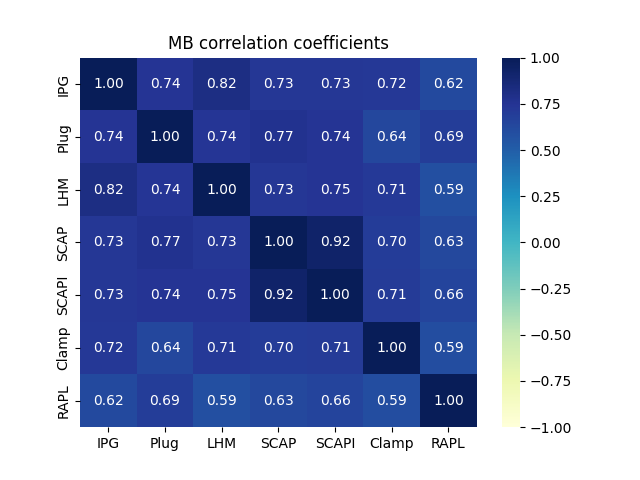
\includegraphics[width=0.6\textwidth]{figures/MandelbrotDut1.png}
    \caption{Heatmap showing the correlation coefficient between all of the measurement instruments for MB on dut 1}
    \label{fig:mandelCorrDut1}
\end{figure}

\paragraph{Measuring Instrument Results:} %When analyzing the results, it will be done for DUT 1 using barcharts in \cref{fig:dut-1-compare-mi} as the deviation in the results is limited, where boxplots for boths duts can be found in \cref{app:exp_two}. 
the results for this experiment, is presented in \cref{fig:dut-1-compare-mi}. In \cref{fig:dut-1-compare-mi}, MB was found to consume less energy than FR for Windows, where the opposite was the case for Linux. When comparing the different software measuring instruments for Windows, SCAP, IPG and LHM were in all cases within $25$ joules of each other, where IPG reported the lowest DEC and SCAPI reported the highest DEC. When the hardware measuring instruments were compared, the Plug reported a higher DEC than the Clamp in all cases. Between OSs, Linux reported a lower DEC for FR, but a higher DEC for MB for both the Clamp and Plug, where RAPL over reports compared to the Clamp in all cases, which was also found on Windows for all measuring instruments.

% In \cref{fig:dut-1-compare-mi}, MB had a lower energy consumption than FR for all measuring instruments except RAPL, where SCAP, LHM and IPG had measurements within 25 joules of each other. When comparing hardware measuring instruments, the Clamp 



% The Clamp (W) measurements are lower than the Plug (W) on both benchmarks, while compared to SCAP, SCAPI, LHM and IPG it is lower for \texttt{MB}, but higher for \texttt{FR}. When comparing between OSs, Windows can be observed to have a lower DEC and Linux. Boxplots for both DUTs can be found in \cref{app:exp_two}.



When the statistical method from \cref{subsec:Statistics} were applied, the data was was found not to follow a normal distribution, was was also found in \cite{biksbois, Koedijk2022diff}.% Thus, Kendall's Tau Correlation Coefficient was used.%, and the results for the two benchmarks can be seen in \cref{fig:fannkuchCorr} and \cref{app:cor_exp_two}.


The correlation between the measuring instruments for MB on DUT 1 can be seen in \cref{fig:mandelCorrDut1}, where it was found that all software based measuring instruments had a moderate to high correlation between $0.59$ - $0.72$ to the Clamp, when assessed with the Guildford Scale. The Plug was found to have a moderate correlation of $0.64$ to the Clamp. The correlations for FR were found to be more correlated compared to MB, but still within the same categories of either a moderate or high correlation, except for on linux on DUT1. All of the correlation results can be found in \cref{app:cor_exp_two}. The similar correlation between the different software based measuring instruments was expected, because of them using the same hardware counters and MSRs. When choosing the best measuring instrument, SCAP and SCAPI were excluded despite a high correlation given a low sample rate and a tedious setup process. Between IPG and LHM, the performance was equal, where IPG was more correlated on MB and LHM on FR. The choice ended up being on IPG, given a better user experience. 


% For the remaining experiments, we chose the software-based instrument based on considerations of accuracy, ease of use, and availability as expressed in \cref{RQ:RQ2}. While SCAPI had the highest correlation on both MB and FR, it and SCAP had a low sample rate and was tedious to set up on Windows, therefore it is not picked. LHM and IPG were close as IPG was slightly more correlated with the Clamp (W) on MB, but slightly less on FR. However, LHM had more problems in the setup phase than IPG and also required calculations for getting the measurements in joules, therefore, we chose IPG. %One thing to note is that our determination of accuracy is based of the accuracy of the Clamp, which means that if the Clamp is not accurate, then we do not know if the other measuring instruments are.